% Analysis Zusammenfassung aus dem Informatikstudium an der ETH Zuerich
% Copyright (C) 2003  Patrick Pletscher

%This program is free software; you can redistribute it and/or
%modify it under the terms of the GNU General Public License
%as published by the Free Software Foundation; either version 2
%of the License, or (at your option) any later version.

%This program is distributed in the hope that it will be useful,
%but WITHOUT ANY WARRANTY; without even the implied warranty of
%MERCHANTABILITY or FITNESS FOR A PARTICULAR PURPOSE.  See the
%GNU General Public License for more details.

%You should have received a copy of the GNU General Public License
%along with this program; if not, write to the Free Software
%Foundation, Inc., 59 Temple Place - Suite 330, Boston, MA  02111-1307, USA.
\documentclass[10pt, a4paper, twocolumn]{scrartcl}

\usepackage{german}
\usepackage{amsmath}
\usepackage{amsfonts}
\usepackage{graphicx}
\usepackage[pageanchor=false,colorlinks=true,urlcolor=black,hyperindex=false]{hyperref}

\textwidth = 16.5 cm
\textheight = 25 cm
\oddsidemargin = 0.0 cm
\evensidemargin = 0.0 cm
\topmargin = 0.0 cm
\headheight = 0.0 cm
\headsep = 0.0 cm
\parskip = 0 cm
\parindent = 0.0cm

% Tiefe des Inhaltsverzeichnisses
\setcounter{secnumdepth}{2}
\setcounter{tocdepth}{2}

\title{Algebra I - Zusamenfassung}
\author{Patrick Pletscher}
\begin{document}

\maketitle

\section{Lineare Gleichungssysteme - Gauss-Elimination}

Ein lineares Gleichungssystem heisst {\bf homogen}, falls die rechte Seite aus Nullen besteht. Andernfalls heisst es inhomogen. Die L"osung $x_1=x_2=\ldots=x_n=0$ eines Systems heisst {\bf triviale} L"osung.\\\\

n: Anzahl Unbekannter, m: Anzahl Gleichungen, r: Zahl bei der Gaussalgorithmus abbricht = Rang des Systems \\

Ein homogenes Gleichungssystem hat genau dann nichttriviale L"osungen, wenn $r < n$ ist. Dann gibt es eine (n-r)-parametrige L"osungsschar.\\
Insbesondere hat ein homogenes System mit $m < n$, d.h mit mehr Unbekannten als Gleichungen, stets eine mindestens (n-m)-parametrige Schar nichttrivialer L"osungen.\\\\

Falls r:=Rang A=n, dann ist A {\bf regul"ar}, falls r:=Rang $A<n$, dann ist A {\bf singul"ar}.\\


\section{Matrizen und Vektoren in $\mathbb{R}^n$ und $\mathbb{C}^n$}

\subsection{Das Rechnen mit Matrizen und Vektoren}
Eine $m\times n$- Matrix A kann mit einer $n\times p$- Matrix B {\bf multipliziert} werden.\\
Das Element $(AB)_{ij}$ in der i-ten Zeile und der j-ten Spalte von AB bekommt man also, indem man die i-te Zeile der Matrix A mit der j-ten Kolonne der Matrix B multipliziert, wobei man die Zeile als Zeilenvektor auffasst und die Kolonne als Kolonnenvektor.\\\\

Ist A eine $m \times n$- Matrix und B=( $b_1$ $b_2$ $\ldots$ $b_p$) eine $n \times p$- Matrix, so gilt:\\
AB = ($Ab_1$ $Ab_2$ \ldots $Ab_p$)\\\\

Das Gleichungssystem {\bf Ax = b} hat genau dann eine L"osung, wenn {\bf b} eine Linearkombination der Kolonnen von A ist.\\

\subsection{Die Transponierte einer Matrix; symmetrische und Hermitesche Matrizen}

Definition:\\
Ist A eine $m\times n$- Matrix, so heisst die $n \times m$- Matrix $A^T$ mit $(A^T)_{ij}:=(A)_{ji}$ die zu A {\bf transponierte} Matrix.\\
Ist A eine komplexe Matrix, so ist $\overline{A}$ mit $(\overline{A})_{ij}:=\overline{(A)_{ij}}$ die zu A konjugiert-komplexe Matrix, und $A^H:=(\overline{A})^T=\overline{A^T}$ ist die zu A konjugiert-transponierte oder Hermitesch-transponierte Matrix.\\\\

Beispiel:\\

A=
$
\left (
\begin{array}{cccc}
1 & 2 & 3 & 4\\
5 & 6 & 7 & 8 
\end{array}
\right )
$

$A^T$=
$
\left (
\begin{array}{cc}
1 & 5\\
2 & 6\\
3 & 7\\
4 & 8
\end{array}
\right )
$\\\\

Eine Matrix A heisst {\bf symmetrisch}, falls $A^T=A$, eine Matrix heisst {\bf Hermitesch}, falls $A^H=A$\\\\

F"ur das Transponieren (auch f"ur $A^H$) gelten folgende Rechenregeln:\\
$(A^T)^T=A$\\
$(\alpha A)^T=\alpha A^T$\\
$(A+B)^T=A^T+B^T$\\
$(AB)^T=B^TA^T$\\\\

F"ur beliebige quadratische Matrizen gilt:\\
A,B symmetrisch, AB=BA $\rightarrow$ AB symmetrisch\\
A,B Hermitesch, AB=BA $\rightarrow$ AB Hermitesch\\\\

F"ur beliebige Matrizen gilt:\\
$A^TA$ und $AA^T$ sind symmetrisch\\
$A^HA$ und $AA^H$ sind Hermitesch\\\\


\subsection{Das Skalarprodukt und die Norm von Vektoren; L"angen und Winkel}

Definition:\\
Das (Euklidische) {\bf Skalarprodukt} oder {\bf innere Produkt} zweier Vektoren $x,y\in \mathbb{E}^n$ ist die Zahl $\langle x,y \rangle$ definiert durch:\\
$\langle x,y \rangle\: :=\: x^Hy=\sum^n_{k=1}\overline{x_k}y_k$\\\\

Die {\bf L"ange} oder 2-Norm oder Euklidische {\bf Norm} eines Vektors $x\in\mathbb{E}^n$ ist die nichtnegative reelle Zahl $\|x\|$ definiert durch $\|x\|:=\sqrt{\rangle x,x \langle}$\\\\

Es gilt die {\bf Schwarzsche Ungleichung}:\\
$|\rangle x,y \langle |\leq\|x\|\:\|y\|$\\\\

$\cos\phi=\frac{Re \langle x,y \rangle}{\|x\|\:\|y\|}$\\\\

\subsection{Das "aussere Produkt und die orthogonale Projektion auf eine Gerade}

Das dyadische Produkt oder {\bf "aussere Produkt} eines m-Vektors x und eines n-Vektors y ist die $m \times n$-Matrix $xy^H$.\\\\

Die orthogonale {\bf Projektion $P_yx$} des n-Vektors x auf die durch die Vielfachen von y ($\neq$ o) erzeugte Gerade durch den Ursprung ist gegeben durch {\bf $P_yx:=\frac{1}{\|y\|^2}yy^Hx$}\\\\

\subsection{Die Inverse einer Matrix}

Eine $n\times n$ Matrix A heisst invertierbar, falls es eine $n\times n$-Matrix X gibt, so dass $AX=I_n=XA$ ist. Die Matrix X heisst Inverse von A und wird mit $A^{-1}$ bezeichnet: $AA^{-1}=I_n=A^{-1}A$.\\
Falls A regul"ar ist, dann ist A auch invertierbar.\\\\

Ist A regul"ar, so hat das Gleichungssystem Ax=b f"ur jede rechte Seite b eine eindeutige L"osung, und zwar ist $x=A^{-1}b$\\\\

\subsection{Orthogonale und unit"are Matrizen}

Eine $n\times n$- Matrix A heisst {\bf unit"ar}, falls $A^HA=I_n$. Eine reelle unit"are Matrix heisst auch {\bf orthogonal}; f"ur sie gilt $A^TA=I_n$.\\\\
Sind A und B unit"are $n\times n$-Matrizen, so gilt:\\
- A ist regul"ar und $A^{-1}=A^H$\\
- $AA^H=I_n$\\
- $A^{-1}$ ist unit"ar
- AB ist unit"ar\\\\

{\bf Householder-Matrizen}\\
Spezielle Klasse orthogonaler Matrizen. Sie beschreiben die Spiegelung an einer Hyperebene, d.h. einer Geraden, falls n=2, und an einer Ebene, wenn n=3.\\
Es sei u eine reeller Kolonnenvektor der L"ange 1, d.h. $u^Tu=1$. Dann ist das "aussere Produkt $uu^T$ ja die $n\times n$-Matrix. Die zu u geh"orende Householder-Matrix ist \\
{\bf $Q_u:=I-2uu^T$}\\
Sie l"asst sich durch die Projektion auf die Richtung u ausdr"ucken (wobei jetzt u reell und $\|u\|=1$ ist):\\

$Q_u=I-2P_u$, wo $P_u=uu^T$\\

$P_u$ und damit auch $Q_u$ symmetrisch.\\

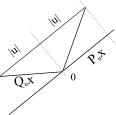
\includegraphics{pictures/householder.png}\\

Die durch eine orthogonale oder unit"are $n \times n$ Matrix A definierte Abbildung ist l"angen und winkeltreu.\\

\section{Die LR-Zerlegung}

\subsection{Die Gauss-Elimination als LR-Zerlegung}

$A=LR$\\\\

Durch die Gauss-Elimination wird also die Koeffizientenmatrix A eines linearen Gleichungssystem implizit in ein Produkt einer Linksdreiecksmatrix L und einer Rechtsdreiecksmatrix R zerlegt. Man nennt deshalb diesen Hauptteil der Gauss-Elimination auch LR-Zerlegung.\\\\

{\bf Zeilenweise, direkte LR-Zerlegung, regul"arer Fall}\\
Zur LR-Zerlegung einer regul"aren Matrix A berechne man f"ur i=1,...,n, mit $l_{ii}:=1$,\\
$l_{ik}:=(a_{ik}-\sum^{k-1}_{j=1}l_{ij}r_{jk})\frac{1}{r_{kk}}\:\: (k=1,\ldots,i-1)$,\\
$r_{ik}:=(a_{ik}-\sum^{i-1}_{j=1}l_{ij}r_{jk})\frac{1}{l_{ii}}\:\: (k=i,\ldots,n)$.\\\\

Danach:\\
- Vorw"artseinsetzen: Lc=b aufl"osen nach c.\\
- R"uckw"artseinsetzen: Rx=c aufl"osen nach x.\\\\

\subsection{Die Cholesky-Zerlegung}

$A=\widetilde{R}^H\widetilde{R}$\\\\

Eine reelle $n\times n$ Matrix, heisst {\bf positiv definit}, wenn:\\
$x^HAx>0$\:\:$x\in\mathbb{R}^n$\\\\

{\bf Zeilenweise, direkte Cholesky-Zerlegung}:\\
Zur Cholesky-Zerlegung einer positiv definiten reell symmetrischen oder Hermitschen $n\times n$ Matrix A berechne man f"ur i=1,...,n:\\
$\widetilde{r}_{ii}:=\sqrt{a_{ii}-\sum^{i-1}_{j=1}|\widetilde{r}_{ji}|^2}$,\\
$\widetilde{r}_{ik}:=(a_{ik}-\sum^{i-1}_{j=1}\overline{\widetilde{r}_{ji}}\widetilde{r}_{jk})\frac{1}{\widetilde{r}_{ii}}\:(k=i+1,\ldots,n).$\\
Dabei sind die Summen leer, wenn i=1 ist. Im letzten Schritt mit i=n entf"allt die zweite Formel.\\
Danach:\\
- Vorw"artseinsetzen: $\widetilde{R}^Hc=b$ aufl"osen nach c.\\
- R"uckw"artseinsetzen: $\widetilde{R}x=c$ aufl"osen nach x.\\

\section{Vektorr"aume}

\subsection{Definition}

Ein Vektorraum V "uber $\mathbb{E}$ ist eine nichtleere Menge auf der eine {\bf Addition}\\
$x,y\in V\mapsto x+y\in V$\\
und eine {\bf skalare Multiplikation}\\
$\alpha \in \mathbb{E},x\in V\mapsto \alpha x \in V$\\
definiert sind, wobei folgende Grundregeln gelten:
\begin{description}
 \item[(V1)] $x+y=y+x$
 \item[(V2)] $(x+y)+z=x+(y+z)$
 \item[(V3)] es gibt eine ausgezeichnetes Element $o\in V$  mit $x+o=x $
 \item[(V4)] zu jedem $x\in V$ gibt es ein eindeutig bestimmtes $-x\in V$ mit $x + (-x)=o$
 \item[(V5)] $\alpha(x+y)=\alpha x + \alpha y$
 \item[(V6)] $(\alpha + \beta)x=\alpha x + \beta x$
 \item[(V7)] $(\alpha \beta)x=\alpha(\beta x)$
 \item[(V8)] $1x=x$
\end{description}

\subsection{Unterr"aume, Erzeugendensysteme}

Eine nichtleere Teilmenge U eines Vektorraums V heisst {\bf Unterraum}, falls sie bez"uglich Addition und skalarer Multiplikation abgeschlossen ist.\\\\

Ein Unterraum ist selbst ein Vektorraum.\\\\

Es sei V ein Vektorraum "uber $\mathbb{E}$, und es seien $a_1,\ldots,a_n \in V$ ausgew"ahlte Vektoren. Ein Vektor der Form $x := \alpha_1 a_1+\ldots+\alpha_n a_n=\sum^{n}_{k=1}\alpha_k a_k$ mit $\alpha_1,\ldots,\alpha_n \in \mathbb{E}$ heisst eine Linearkombination von $\alpha_1,\ldots,a_n$.\\\\

Die Menge aller Linearkombinationen von $a_1,\ldots,a_n$ heisst der von $a_1,\ldots,a_n$ aufgespannte/erzeugte Unterraum. Er wird bezeichnet mit $span\{a_1,\ldots,a_n\}$\\

\subsection{Lineare Abh"angigkeit, Basen, Dimension}

Die $n\geq 2$ Vektoren $a_1,\ldots,a_n$ sind {\bf linear abh"angig} genau dann, wenn sich einer dieser Vektoren als Linearkombination der andern schreiben l"asst.\\\\

Ein linear unabh"angiges Erzeugendensystem eines Vektorraums V heisst Basis von V.\\\\

${b_1,\ldots,b_m}\subset V$ ist genau dann eine Basis von V, wenn sich jeder Vektor $x \in V$ in eindeutiger Weise als Linearkombination von $b_1,\ldots,b_m$ darstellen l"asst. $x=\sum^m_{k=1}\xi_k b_k$\\

Testen auf lin. Abh"angigkeit: $\alpha v_1 +\beta v_2 +\gamma v_3=0$ 


\subsection{Basiswechsel, Koordinatentransformation}

Es sei ${b_1,\ldots,b_n}$ eine vorgegebene, alte Basis des Vektorraumes V, und es sei ${b'_1,\ldots,b'_n}$ eine zweite, neue Basis von V. Die neuen Basisvektoren kann man in der alten Basis darstellen:$b'_k=\sum^n_{i=1}\tau_{ik}b_i\:\: (k=1,\ldots,n)$\\

Die $n \times n$-Matrix $T = (\tau_{ik})$ heisst Transformationsmatrix des Basiswechsels.\\
$
\left. \xi
\begin{array}{c}
 T^{-1}\\
 \rightarrow\\
 \leftarrow\\
 T
\end{array}
\xi' \right.
$\\

Es sei $\xi=(\xi_1\:\ldots\:\xi_n)^T$ der Koordinatenvektor eines beliebigen Vektors $x \in V$ bez"uglich der alten Bais, und es sei $\xi'=(\xi'_1\:\ldots\:\xi'_n)^T$ der Koordinatenvektor dieses Vektors x bez"uglich einer neuen, gegebenen Basis, so dass\\
$\sum^n_{k=1}\xi_k b_k=x=\sum^n_{k=1}\xi'_kb'_k$\\
Dann gilt f"ur die Koordinatentransformation:
$\xi_i=\sum^n_{k=1}\tau_{ik}\xi'_k\:\:(i=1,\ldots,n)$\\
d.h. es ist $\xi=T\xi'$\\
wobei die Transformationsmatrix T regul"ar ist, so dass also\\
$\xi'=T^{-1}\xi$

\section{Lineare Abbildungen}

\subsection{Definition, Matrixdarstellung}

Eine Abbildung $F:X\rightarrow Y, x \mapsto Fx$ zwischen zwei Vektorr"aumen X und Y ("uber $\mathbb{E}$ heisst {\bf linear}, wenn f"ur alle $x,\widetilde{x}\in X$ und alle $\gamma\in\mathbb{E}$ gilt\\
$F(x+\widetilde{x})=Fx+F(\widetilde{x}),\:\:\:\:F(\gamma x)=\gamma(Fx)$\\
X ist der Definitionsraum, Y der Bildraum der Abbildung.

Wir betrachten nun eine beliebige lineare Abbildung F eines n-dimensionalen Vektorraums X in einen m-dimensionalen Vektorraum Y. Es sei ${b_1,\ldots,b_n}$ eine Basis von X, ${c_1,\ldots,c_m}$ eine Basis von Y.\\
Die Bilder $Fb_l \in Y$ der Basis von X lassen sich als Linearkombinationen der $c_k$ darstellen:\\
$Fb_l=\sum^m_{k=1}a_{kl}c_k\:\:\:\:(l=1,\ldots,n)$\\
Die $m\times n$-Matrix $A=(a_{kl})$ heisst Abbildungsmatrix von F bez"uglich den gegebenen Basen in X und Y.\\\\

$x\in X$:\\
$x=\sum^n_{l=1}\xi_l b_l$\\
mit dem Koordinatenvektor $\xi:= (\xi_1\:\ldots\:\xi_n)^T$.\\\\

$y\in Y$:\\
$y=\sum^m_{k=1}\eta_k c_k$\\
mit dem Koordinatenvektor $\eta:= (\eta_1\:\ldots\:\eta_m)^T$.\\\\

somit gilt: $\eta=A\xi$.\\\\

Eine eineindeutige Abbildung von X auf Y heisst Isomorphismus.\\
Ist $F:X\rightarrow Y$ ein {\bf Isomorphismus}, so ist die inverese Abbildung $F^{-1}:Y\rightarrow X$ linear und auch ein Isomorphismus.\\

\subsection{Kern, Bild und Rang}

Der Kern $ker\:F$ von F ist das Urbild von $o \in Y$. Das Bild $im\:F$ von F ist das Bild des Definitionsraumes X.\\\\

$ker\:F$ ist ein Unterraum von X ($Ax={o}$), und $im\:F$ ist ein Unterraum von Y.\\\\

F ist genau dann injektiv, wenn $ker F = {o}$ ist\\\\

Es gilt die {\bf Dimensionsformel}\\
dim X - dim ker F = dim im F\\\\

Der Rang einer linearen Abbildung F ist gleich der Dimension des Bildes von F:\\
Rang F := dim im F\\

\subsection{Matrizen als lineare Abbildung}

$A=(a_1 a_2 \ldots a_n)$\\\\

Der von den Kolonnen von A aufgespannte Unterraum $\mathcal{R}(A)$ := $span\{a_1,\ldots,a_n\}$ heisst Kolonnenraum oder Wertebereich von A. Der L"osungsraum $\mathcal{L}_0$ des homogenen Systems Ax=o heisst Nullraum $\mathcal{N}(A)$.\\\\

Fasst man die Matrix A als lineare Abbildung auf, so ist das Bild von A gleich dem Kolonnenraum oder Wertebereich von A, und der Kern von A ist gleich dem Nullraum von A:\\ im A = $\mathcal{R}(A)$, \ \ \ ker A = $\mathcal{N}(A)$.\\

Das Gleichungssystem Ax=b ist genau dann l"osbar, wenn b im Kolonnenraum von A liegt. Eine allf"allige L"osung ist genau dann eindeutig, wenn $\mathcal{N}$(A)={o} ist, das heisst das homogene System nur die triviale L"osung hat.\\\\

Bezeichnet r den Rang der Matrix A und $\mathcal{L}_0$ den L"osungsraum von Ax=o, so ist

dim $\mathcal{L}_0$= dim $\mathcal{N}(A)$ = dim ker A = n-r\\\\

{\bf Der Rang einer $m \times n$ Matrix A ist gleich}\\
\begin{description}
 \item[(1)] der Anzahl Pivotelemente bei der Reduktion von A auf Zeilenstufenform.
 \item[(2)] dem Rang der linearen Abbildung A: $\mathbb{E}^n\rightarrow\mathbb{E}^m$, definiert als dim im A
 \item[(3)] der Dimension des Kolonnenraums (Kolonnenrang), definiert als Anzahl linear unabh"angiger Kolonnen ($\in \mathbb{E}^n$)
 \item[(4)] der Dimension des Zeilenraums (Zeilenrang), definiert als Anzahl linear unabh"angiger Zeilen ($\in \mathbb{E}^n$).
\end{description}

\subsection{Die Abbildungsmatrix bei Koordinatentransformation}

$\xi \in \mathbb{E}^n$\ \ \ \ \ \ \ \ A \ \ \ \ \ \ \ \ $\eta \in \mathbb{E}^m$\\
$T^{-1}\downarrow\uparrow T$\ \ \ \ \ \ \ \ \ \ \ \ \ $S^{-1}\downarrow \uparrow S$\ \ (Koordinatentrans.)\\
$\xi' \in \mathbb{E}^n$\ \ \ \ \ \ \ \ B \ \ \ \ \ \ \ \ $\eta' \in \mathbb{E}^m$\\\\

$B=S^{-1}AT$, \ \ $A=SBT^{-1}$\\

\section{Vektorr"aume mit Skalarprodukt}


\subsection{Vektorr"aume mit Skalarprodukt}

Die Norm oder L"ange eines Vektors x in einem Vektorraum V mit Skalarprodukt ist\\
$\|x\|\equiv\sqrt{\langle x,x \rangle}$\\\\

Der Winkel zwischen zwei Vektoren x und y ist gegeben durch\\
$\varphi =\angle(x,y)\equiv \arccos\frac{Re\:\langle x,y \rangle}{\|x\|\|y\|}$\\\\


{\bf Satz von Pythagoras}\\
In einem Vektorraum mit Skalarprodukt gilt:\\
$x\bot y \:\Rightarrow\:\|x\pm y\|^2=\|x\|^2+\|y\|^2$

\subsection{Orthonormalbasen}

Ist V ein n-dimensionaler Vektorraum mit Skalarprodukt und ${b_1,\ldots,b_n}$ eine Orthonormalbasis, so gilt f"ur jedes $x \in V$\\
$x=\sum^n_{k=1}\langle b_k,x \rangle b_k$\\\\

{\bf Gram-Schmidt-Orthogonalisierungsverfahren}\\
Es sei ${a_1,a_2,\ldots}$ eine endliche oder abz"ahlbare, linear unabh"angige Menge von Vektoren. Wir berechnen eine gleich grosse Menge ${b_1,b_2,\ldots}$ von normierten und paarweise orthogonalen Vektoren rekursiv gem"ass.\\
{\bf
$b_1 \equiv\frac{a_1}{\|a_1\|}$,\\
$\widetilde{b}_k\equiv a_k - \sum^{k-1}_{j=1}\langle b_j, a_k \rangle b_j$,\\
$b_k\equiv\frac{\widetilde{b}_k}{\|\widetilde{b}_k\|}$
}

\subsection{Orthogonale und unit"are Basiswechsel und Koordinatentransformationen}

Die Transformationsmatrix einer Basistransformation zwischen orthonormierten Basen ist unit"ar ($I=T^H T$). Dadurch sind die alten und neuen Koordinatenvektoren $\xi$ und $\xi'$ verkn"upft gem"ass:\\
$\xi=T\xi',\:\:\:\xi'=T^H\xi$

\subsection{Orthogonale und unit"are Abbildungen}

Es seien X und Y zwei unit"are (bzw. orthogonale) Vektorr"aume. Eine lineare Abbildung F:X $\rightarrow$ Y heisst unit"ar (bzw. orthogonal), falls f"ur x,y $\in$ X gilt:\\
$\langle Fx,Fy \rangle_Y=\langle x,y\rangle_X$\\
Eine solche Abbildung ist l"angen- und winkeltreu, zus"atzlich ist ker F =${o}$, d.h. F ist injektiv.

\subsection{Normen von linearen Abbildungen (Operatoren) und Matrizen}

X und Y zwei normierte Vektorr"aume. Eine lineare Abbildung F:X $\rightarrow$ Y heisst beschr"ankt, wenn es ein $\gamma_F\geq0$ gibt mit $\|F(x)\|_Y\leq\gamma_F\|x\|_X\:\:(\forall x \in X)$ 



\section{Die Methode der kleinsten Quadrate und die QR-Zerlegung einer Matrix}

\subsection{Orthogonalprojektionen}

Eine lineare Abbildung $P:\:\mathbb{E}^m\rightarrow\mathbb{E}^m$ heisst Projektion oder Projektor, falls $P^2=P$\\
Eine Projektion heisst Orthogonalprojektion oder orthogonaler Projektor, falls zus"atzlich gilt ker P $\bot$ im P.\\
Ist P ein Projektor, so ist auch I-P ein Projektor und es gilt:\\
im(I-P) = ker P, ker(I-P) = im P\\\\

F"ur einen Projektor $P: \mathbb{E}^m\:\rightarrow\:\mathbb{E}^m$ sind folgende Aussagen "aquivalent:\\
- P ist ein orthogonaler Projektor\\
- I - P ist ein orthogonaler Projektor\\
- $P^H=P$\\\\


Sind die Kolonnen einer $m\times n$-Matrix A linear unabh"angig, d.h. ist Rang A = n ($\leq m$), so ist $A^HA$ regul"ar.\\\\


Die Orthogonalprojektion $P_A:\mathbb{E}^m\:\rightarrow\:im\:A \subseteq \mathbb{E}^m$ auf den Kolonnenraum $\mathcal{R}(A)$=im A einer $m\times n$-Matrix A mit Rang n($\leq m$) ist gegeben durch\\
$P_A\equiv A(A^HA)^{-1}A^H$\\
also $P_A y$\\
{\bf $P_A y=A(A^HA)^{-1}A^Hy$}\\

wenn Kolonnen von Q orthogonal\\
$P_Q\equiv QQ^H$


\subsection{Die Methode der kleinsten Quadrate}

"Uberbestimmtes lineares Gleichungssystem Ax=y mit einer ''hohen'' $m\times n$-Matrix $(m>n)$. Hat im allgemeinen keine L"osungen.\\
Wenn keine L"osung, dann x so w"ahlen, dass Residuenvektor $(r\equiv y-Ax)$ minimale Euklidische Norm hat:\\
$\|r\|^2=\sum^{m}_{k=1}r^2_k$\\
$x=(A^HA)^{-1}A^Hy$ oder $A^TA\vec{x}=A^T\vec{y}$


\subsection{Die QR-Zerlegung einer Matrix}

Das Gram-Schmidt-Verfahren, angewandt auf die Kolonnen $a_1,\ldots,a_n$ einer $m\times n$-Matrix A liefert die QR-Faktorisierung dieser Matrix. Erg"anzt man A durch den m-Vektor y, so liefert das Verfahren (vor dem Normieren) zus"atzlich den $\mathcal{R}(A)$ orthogonalen Residuenvektor r gem"ass der Formel\\
$r=y-QQ^Hy$\\
Die L"osung x des Kleinste-Quadrate-Problems erf"ullt das durch R"uckw"artseinsetzen l"osbare System $Rx=Q^Hy$.

\subsection{Die QR-Zerlegung mit Pivotieren}

modifiziertes Gram-Schmidt-Verfahren mit Kolonnen-Pivotieren\\
$q_1:=\frac{a_1}{\|a_1\|},\:\:\:\widetilde{q_i}\equiv a_i - q_1\langle q_1,a_i \rangle$\\
w"ahle $p \geq k$ mit $\|\widetilde{q_p}\|\neq 0$ und vertausche Kolonnen p und k; berechne\\
$q_k:=\frac{\widetilde{q_k}}{\|\widetilde{q_k}\|}$,\\
$\widetilde{q_i}:=\widetilde{q_i}-q_k\langle q_k,\widetilde{q_i}\rangle\:\:(i=k+1,\ldots,n)$;\\
ist $\|\widetilde{q_{k+1}}=\ldots=\|\widetilde{q_n}\|=0$, so gilt Rang A = k und man ist fertig.


\section{Determinaten}

\subsection{Definition, Eigenschaften}

Regel von Sarrus:\\
$
\left \bracevert
\begin{array}{ccc}
a_{11} & a_{12} & a_{13}\\
a_{21} & a_{22} & a_{23}\\
a_{31} & a_{32} & a_{33}
\end{array}
\right \bracevert
=a_{11}a_{22}a_{33}+a_{21}a_{32}a_{13}+a_{31}a_{12}a_{23}-a_{31}a_{22}a_{13}-a_{21}a_{12}a_{33}-a_{11}a_{32}a_{23}$\\\\

Eine Determinante ist ein Funktional $(A\mapsto det A)$ mit den folgenden Eingenschaften:\\
\begin{description}
 \item[-] det ist eine lineare Funktion jeder einzelnen Zeile/Kolonne der Matrix\\
\tiny
$
det \left (
\begin{array}{ccc}
a_{11} & \ldots & a_{1n}\\
\vdots &        & \vdots\\
\gamma a_{l1} + \gamma' a'_{l1} & \ldots & \gamma a_{ln} +\gamma' a'_{ln}\\
\vdots &        & \vdots\\
a_{n1} & \ldots & a_{nn}
\end{array}
\right )\\
=\gamma 
det \left (
\begin{array}{ccc}
a_{11} &  \ldots & a_{1n}\\
\vdots &         & \vdots\\
a_{l1} &  \ldots & a_{ln} \\
\vdots &         & \vdots\\
a_{n1} &  \ldots & a_{nn}
\end{array}
\right )
+\gamma' 
det \left (
\begin{array}{ccc}
a_{11} &  \ldots & a_{1n}\\
\vdots &         & \vdots\\
a'_{l1} &  \ldots & a'_{ln} \\
\vdots &         & \vdots\\
a_{n1} &  \ldots & a_{nn}
\end{array}
\right )
$
\normalsize
 \item[-] Werden in A zwei Zeilen/Kolonnen vertauscht, so wechselt det(A) das Vorzeichen
 \item[-] det(I)=1
 \item[-] Hat A eine Zeile/Kolonne aus lauter Nullen, so ist det A=0
 \item[-] $det(\gamma A)=\gamma^n det A$\\
 \item[-] Hat A zwei gleiche Zeilen/Kolonnen, so ist det A=0\\
 \item[-] Addiert man zu einer Zeile/Kolonne von A ein Vielfaches einer anderen Zeile/Kolonne von A, so "andert sich der Wert von det A nicht.
 \item[-] Ist A eine Diagonalmatrix, so ist det A gleich dem Produkt der Diagonalelemente.
 \item[-] Ist A eine Dreiecksmatrix, so ist det A gleich dem Produkt der Diagonalelemente.
\end{description}

\tiny
$ 
det \left (
\begin{array}{ccc}
a_{11} &  \ldots & \gamma a_{1n}\\
\vdots &         & \vdots\\
a_{n1} &  \ldots & \gamma a_{nn}
\end{array}
\right )
=
\gamma det \left (
\begin{array}{ccc}
a_{11} &  \ldots & a_{1n}\\
\vdots &         & \vdots\\
a_{n1} &  \ldots & a_{n}
\end{array}
\right )
$\normalsize\\\\


F"ur jede $n\times n$ Matrix A gilt:\\
$det\:A \neq 0\: \Leftrightarrow\:Rang A = n \:\Leftrightarrow\:$A ist regul"ar\\

Wendet man auf A den {\bf Gauss-Algorithmus} an und ist dabei Rang A=n, so ist {\bf det A gleich dem Produkt der Pivotelemente} multipliziert mit $(-1)^\nu$, wobei $\nu$ die Anzahl der ausgef"uhrten Zeilenvertauschungen bezeichnet:\\
$det\:A = (-1)^\nu \Pi^n_{k=1}r_{kk}$\\\\

\textbf{Determinante via Gauss-Algorithmus}\\
Zur Berechnung der Determinante einer $n\times n$-Matrix A wende man den Gauss-Algorithmus auf A an. Falls er den Rang n und die obere Dreiecksmatrix R liefert, so gilt obere Formel. Ist Rang A $<$ n, so ist det A = 0.\\\\

F"ur irgend zwei $n\times n$-Matrizen A und B gilt:\\
$det(AB)=det\:A \cdot det\:B$\\\\

Ist A regul"ar, so gilt:\\
$det\:A^{-1}=(det\:A)^{-1}$\\
$det\:A^{n}=(det\:A)^{n}$\\\\

Es gilt:\\
$det\:A^T = det\:A\:\:\:\:det\:A^H=\overline{det\:A}$

\subsection{Entwicklung nach Zeilen und Kolonnen}

Zu jedem Element $a_{kl}$ einer $n\times n$-Matrix A werde die $(n-1)\times(n-1)$-Untermatrix $A_{[k,l]}$ definiert durch Streichen der Zeile k und der Kolonne l von A. Der Kofaktor $\kappa_{k,l}$ von $a_{kl}$ ist dann eine Zahl\\
$\kappa_{k,l}:\equiv(-1)^{k+l}det\:A_{[k,l]}$\\\\

Entwicklung nach der k-ten Zeile (k fest):\\
$det\:A=\sum^n_{i=1}a_{ki}\kappa_{ki}$\\\\

Entwicklung nach der l-ten Kolonne (l fest):\\
$det\:A=\sum^n_{i=1}a_{il}\kappa_{il}$


\subsection{Determinanten von Blockdreiecksmatrizen}

$
\left \bracevert
\begin{array}{cc}
A & B \\
O & D 
\end{array}
\right \bracevert
=det\:A\:det\:D
$
$
\left \bracevert
\begin{array}{cc}
A & O \\
C & D 
\end{array}
\right \bracevert
=det\:A\:det\:D
$


\section{Eigenwerte und Eigenvektoren}

$\lambda $ ist genau dann ein Eigenwert von $A \in \mathbb{E}^{n\times n}$, wenn $A-\lambda I$ singul"ar ist.$(det (A-\lambda I)=0)$\\
Der Eigenraum $E_\lambda$ zu einem Eigenwert $\lambda$ von A ist ein vom Nullraum verschiedener Unterraum des $\mathbb{E}^n$, und zwar ist\\
$E_\lambda=ker(A-\lambda I)$,\\
das heisst $E_\lambda$ besteht aus allen L"osungen v des homogenen Gleichungssystems\\
$(A-\lambda I)v=o$\\
Die {\bf geometrische Vielfachheit} von $\lambda$ betr"agt\\
$dim\:E_\lambda = dim\:ker(A-\lambda I)= n - Rang(A-\lambda I)$\\\\

Das Polynom $\chi_A(\lambda):\equiv det(A-\lambda I)$ heisst {\bf charakteristisches Polynom} der Matrix $A \in \mathbb{E}^{n\times n}$, und die Gleichung $\chi_A(\lambda)=0$ ist die charakteristische Gleichung.\\\\

$\lambda \in \mathbb{E}$ ist genau dann Eigenwert der der Matrix $A \in \mathbb{E}^{n\times n}$, wenn $\lambda$ Nullstelle des charakteristischen Polynoms $\chi_A$ ist, das heisst eine L"osung der charakteristischen Gleichung ist.\\\\

Berechnung von Eigenwerten und Eigenvektoren via charakteristisches Polynom:\\
Um die Eigenwerte und Eigenvektoren einer Matrix $A \in \mathbb{C}^{n\times n}$ zu bestimmen, kann man theoretisch wie folgt vorgehen:
\begin{description}
 \item[1] Berechnung des charakteristischen Polynoms $\chi_A$,
 $\chi_A(\lambda):\equiv det(A-\lambda I)$
 \item[2] Berechnung der n Nullstellen $\lambda_1,\ldots ,\lambda_n$ von $\chi_A$. Die Vielfachheit einer Nullstelle ist gleich der {\bf algebraischen Vielfachheit} dieses Eigenwertes.
 \item[3] F"ur jeden versch. Eigenwert $\lambda_k$: $A-\lambda_k I$ mit Gauss-Algorithmus auf Zeilenstufenform und w"ahlt von den n-r freien Parametern der Reihe nach immer einen $\neq$ 0 und die anderen 0. Die Dimension n-r des L"osungsraumes ist gleich der {\bf geometrischen Vielfachheit} dieses Eigenwertes.
\end{description}

Eine (quadratische) Matrix A ist genau dann singul"ar, wenn sie 0 als Eigenwert hat.

\subsection{"Ahnlichkeitstransformationen; die Eigenwertzerlegung}

Falls gilt\\
$B=T^{-1}AT,\:\:\:A=TBT^{-1}$\\
A und B sind "ahnlich.\\\\

"Ahnliche Matrizen haben dasselbe charakteristische Polynom; sie haben also die gleiche Determinante, die gleiche Spur und die gleichen Eigenwerte.\\
Sowohl die geometrische als auch die algebraische Vielfachheit eines Eigenwertes ist bei "ahnlichen Matrixen gleich.\\\\

Eine zu $F: V \rightarrow V$ geh"orende Abbildungsmatrix ist genau dann diagonal, wenn die gew"ahlte Basis von V aus lauter Eigenvektoren von F besteht.\\\\

Eine Basis aus Eigenvektoren von F (oder A) heisst Eigenbasis von F (bzw. A).\\
Gibt es eine Eigenbasis $v_1,\ldots,v_n$ so gilt also die einfache Abbildungsformel\\
$x=\sum^n_{k=1}\xi_k v_k\:\mapsto\:Fx=\sum^n_{k=1}\lambda_k\xi_k v_k$\\\\

{\bf Spektralzerlegung oder Eigenwertzerlegung}\\
Zu einer Matrix $A \in \mathbb{E}^{n\times n}$ gibt es genau dann eine "ahnliche Diagonalmatrix $\Lambda$, wenn es eine Eigenbasis von A gibt. F"ur die regul"are Matrix\\
$V:\equiv(v_1\:\ldots\:v_n)$\\
mit dieser Eigenbasis als Kolonnen gilt dann\\
$AV=V\Lambda$, d.h. $A=V\Lambda V^{-1}$ bzw. {\bf $\Lambda=V^{-1}AV$}\\
Gibt es umgekehrt eine regul"are Matrix $V \in \mathbb{E}^{n\times n}$ und eine Diagonalmatrix $\Lambda \in \mathbb{E}^{n \times n}$, so dass obiger Satz gilt, so sind die Diagonalelemente von $\Lambda$ Eigenwerte von A und die Kolonnen von V entsprechende Eigenvektoren, die eine Eigenbasis bilden.\\
Eine Matrix A, zu der es eine Spektralzerlegung $A=V\Lambda V^{-1}$ mit diagonalem $\Lambda$ gibt, heisst diagonalisierbar.\\\\

Ist A diagonalisierbar und zerlegen wir die Matrizen V und $V^{-1}$ aus der Spektralzerlegung $A=V\Lambda V^{-1}$ in Kolonnen bzw. Zeilenvektoren,\\
$V=(\:v_1\:\ldots\:v_n)$
$V^{-1}=
\left ( 
\begin{array}{c}
w^T_1 \\
\vdots \\ 
w^T_n
\end{array}
\right )
$\\

so l"asst sich A als Summe von n Rang-1-Matrizen darstellen:\\
$A=\sum^n_{k=1}v_k \lambda_k w_k^T$\\
Dabei gilt $Av_k=v_k\lambda_k$ und $w^T_kA=\lambda_k w^T_k$\\\\


Eigenvektoren zu verschiedenen Eigenwerten sind linear unabh"angig.\\\\

Sind die n Eigenwerte von $F:V\rightarrow V$ (wo n=dim V) verschieden, so gibt es eine Basis von Eigenvektoren und die entsprechende Abbildungsmatrix ist diagonal.\\\\

F"ur jeden Eigenwert gilt, dass die geometrische Vielfachheit kleiner gleich der algebraischen Vielfachheit ist.\\\\


Eine Matrix ist genau dann {\bf diagonalisierbar}, wenn {\bf f"ur jeden Eigenwert die geometrische gleich der algebraischen Vielfachheit} ist.

\subsection{Eigenwerte und Eigenvektoren symmetrischer und Hermitscher Matrizen}

Ist $A \in \mathbb{C}^{n \times n}$ symmetrisch (Hermitesch), so gilt:\\
\begin{description}
 \item[i)] Alle Eigenwerte $\lambda_1,\ldots,\lambda_n$ sind reell.
 \item[ii)] Die Eigenvektoren zu verschiedenen Eigenwerten sind paarweise orthogonal in $\mathbb{R}^n$ ($\mathbb{C}^n$)
 \item[iii)] Es gibt eine orthogonale Basis des $\mathbb{R}^n$ ($\mathbb{C}^n$) aus Eigenvektoren $u_1,\ldots,u_n$ von A.
 \item[iv)] F"ur die orthogonale (unit"are) Matrix $U :\equiv (u_1\:\ldots\: u_n)$ gilt:\\
  $U^HAU=\Lambda:\equiv diag(\lambda_1,\ldots,\lambda_n)$
\end{description}



\section{Anwendungen der Eigenwertzerlegung}

\subsection{Homogene lineare Differentialgleichungen mit konstanten Koeffizienten}

{\bf Systeme erster Ordnung}\\

Gegeben sei ein System von homogenen linearen Differentialgleichungen erster Ordnung\\
$\dot{y}_1(t)= a_{11}y_1(t) + \ldots + a_{1n}y_n(t)$\\
$\vdots$\\
$\dot{y}_n(t)= a_{n1}y_1(t) + \ldots + a_{nn}y_n(t)$\\
mit konstanten Koeffizienten $a_{kl}$\\
$\eta_1,\ldots,\eta_n$ vorgegebene Zahlen f"ur $y_i(0)$\\
so kann man die Gleichung in Matrixform schreiben:\\
$\dot{y}(t)=Ay(t),\:\:y(0)=y_0$\\
die allgemeine L"osung davon lautet:\\
$y(t)=V e^{t\Lambda}c$\\
$e^{t\Lambda}:\equiv diag(e^{\lambda_1 t},\ldots,e^{\lambda_n t})$\\
$c=(\gamma_1,\ldots,\gamma_n)$\\
mit Anfangsbedingungen:$Vc=y_0\:\:\:c=V^{-1}y_0$\\\\


{\bf Systeme h"oherer Ordnung}\\
$x^{(n)}(t)-\beta_nx^{(n-1)}(t)-\cdots-\beta_2\dot{x}(t)-\beta_1x(t)$\\
mit den Anfangsbedingungen:\\
$x(0)=\eta_1,\:\:,\dot{x}(0)=\eta_2,\:\:\ldots,\:\:x^{(n-1)}(0)=\eta_n$\\
gegeben, so setzen wir\\
$y_1(t):\equiv x(t),\:\:y_2(t):\equiv\dot{x}(t),\:\:\ldots,\:\: y_n(t):\equiv x^{(n-1)}(t)$\\

$A=
\left ( 
\begin{array}{cccc}
0 & 1 & \ldots & 0 \\
\vdots &  & \ddots & \vdots \\
0 & \ldots & 0 & 1 \\
\beta_1 & \beta_2 &\ldots & \beta_n
\end{array}
\right )
$\\\\

{\bf Systeme zweiter Ordnung ohne Terme erster Ordnung}\\
$\ddot{y}_1(t)= a_{11}y_1(t) + \ldots + a_{1n}y_n(t)$\\
$\vdots$\\
$\ddot{y}_n(t)= a_{n1}y_1(t) + \ldots + a_{nn}y_n(t)$\\
mit Anfangsbedingungen:\\
$y_i(0)=\eta_i,\:\:\dot{y}_i(0)=\eta'_i$\\
also:$\ddot{y}(t)=Ay(t),\:\:y(0)=y_0,\:\:\dot{y}(0)=y_1$\\
$\omega_k:\equiv \sqrt{-\lambda_k}$\\
$\Omega:\equiv diag(\omega_1,\ldots,\omega_n)$\\
$\cos(\Omega t):\equiv diag(\cos(\omega_1 t),\ldots,\cos(\omega_n t t)))$\\
$\sin(\Omega t):\equiv diag(\sin(\omega_1 t),\ldots,\sin(\omega_n t t)))$\\
die allgemeine L"osung ist dann:\\
$y(t)=V(\cos(\Omega t)a + \sin(\Omega t)b)$\\
$Va=y_0,\:\:\:V\widetilde{b}=y_1$ mit $\widetilde{b}:\equiv\Omega b$


\subsection{Funktionen von Matrizen}

$f(\Lambda) :\equiv diag (f(\lambda_1),\ldots,f(\lambda_n))$\\
$f(A):\equiv Vf(\Lambda)V^{-1}$


\subsection{Qudratische Formen und ihre Hauptachsentransformation}

Kegelschnitte:\\
$\frac{x_1^2}{a^2}+\frac{x_2^2}{b^2}=1$:  Ellipse mit Halbachsen a und b\\
$\frac{x_1^2}{a^2}-\frac{x_2^2}{b^2}=1$:  Hyperbel mit Halbachse a und Asymptotensteigung $\pm\arctan(b/a)$\\
$x_1^2-2px_2=0$:  Nach oben ge"offnete Parabel mit Halbparameter p\\\\

Eine auf $\mathbb{R}^n \times \mathbb{R}^n$ definierte symmetrische bilineare Form B ist eine Funktion der Form\\
$(x,y)\in \mathbb{R}^n \times \mathbb{R}^n\:\:\mapsto\:\:B(x,y):\equiv x^TAy \in \mathbb{R}$,\\
mit einer reellen, symmetrischen $n \times n$-Matrix A. Die zugeh"orige auf $\mathbb{R}^n$ definierte quadratische Form Q ist\\
$x\in \mathbb{R}^n \:\:\mapsto\:\:Q(x):\equiv x^TAx \in \mathbb{R}$,\\
Eine auf $\mathbb{C}^n \times \mathbb{C}^n$ definierte Hermitesche Form B ist eine Funktion der Form\\
$(x,y)\in \mathbb{R}^n \times \mathbb{R}^n\:\:\mapsto\:\:B(x,y):\equiv x^HAy \in \mathbb{R}$,\\
mit einer Hermitschen $n \times n$-Matrix A.\\\\

Hauptachsendarstellung:\\
$A=U\Lambda U^T,\:\:\widetilde{x}:\equiv U^Tx$\\
$Q(x)=\widetilde{Q}(\widetilde{x}):\equiv\widetilde{x}^T\Lambda\widetilde{x}=\sum^n_{k=1}\lambda_k\widetilde{x}^2_k$\\\\

Jede quadratische Form $Q(x)=x^TAx$ l"asst sich mittels einer auf der Spektralzerlegung von A beruhenden orthogonalen Basistransformation auf die Hauptachsen-Darstellung bringen.\\\\

Jede quadratische Form $Q(x)=x^TAx$ l"asst sich durch "Ubergang auf eine neue orthogonale (aber im allgemeinen nicht orthonormierte) Basis mit Koordinaten y auf die folgende Form bringen:\\
$Q(x)=y^TI_{\pm} y=\sum^p_{k=1}y^2_k-\sum^r_{l=p+1}y^2_l$\\
$I_{\pm}:\equiv (1,\ldots,1,-1,\ldots,-1,0,\ldots,0)$
Die Zahl p ist dabei gleich der Anzahl positiver Eigenwerte von A, und r ist der Rang von A, d.h. r-p ist die Anzahl negativer Eigenwerte.\\\\

Das Tripel (p,r-p,n-r) mit der Zahl der positiven, negativen und null Eigenwerte von A heisst Tr"agheit von A. Die Differenz p-(r-p) der Zahl positiver und negativer Eigenwerte heisst Signatur von A.\\\\

Zwei $n \times n$-Matrizen A und B heissen kongruent, wenn es eine regul"are Matrix S gibt, so dass\\
$A=SBS^T$\\
Der "Ubergang von $B\mapsto A=SBS^T$ (oder umgekehrt) heisst dann Kongruenztransformation.\\\\

Tr"agheitssatz:\\
Zu jeder reellen symmetrischen Matrix A gibt es eine kongruente Matrix $I_{\pm}$. Dabei ist das Tripel (p,r-p,n-r) gleich der Tr"agheit von A, die unabh"angig ist von der zugrunde liegenden Kongruenztransformation.\\\\

Eine symmetrische Matrix ist genau dann positiv definit, wenn all ihre Eigenwerte positiv sind.

\subsection{Die Spektralnorm}

Die Spektralnorm einer Matrix $A \in \mathbb{E}^{n\times n}$ ist gleich der Wurzel aus dem gr"ossten Eigenwert von $A^HA$ $\|A\|_2=\sqrt{\lambda_{max}}$.\\
Die Spektralnorm einer Hermiteschen/symmetrischen Matrix $A \in \mathbb{E}^{n\times n}$ ist gleich dem Betrag des gr"ossten Eigenwerts diser Matrix $\|A\|_2=\lambda_{max}$.\\\\

Die Spektralnorm der Inversen $A^{-1}$ einer Matrix ist gleich dem Inversen der Wurzel aus dem kleinsten Eigenwert von $A^HA$ $\|A^{-1}\|_2 = \frac{1}{\sqrt{\lambda_{min}}}$.\\
Ist A Hermitesch/symmetrisch, so ist $\|A^{-1}\|_2$ gleich dem Inversen des Betrages des kleinsten Eigenwertes von A $\|A^{-1}\|_2 = \lambda_{min}$.\\\\

Die Konditionszahl einer Matrix $A \in \mathbb{E}^{n \times n}$ ist gegeben durch $\kappa_2(A)= \frac{\sqrt{\lambda_{max} von A^HA}}{\sqrt{\lambda_{min} von A^HA}}$.\\
Ist A Hermitesch(symmetrisch), so vereinfacht sich diese Formel zu $\kappa_2(A)= \frac{\lambda_{max} von A}{\lambda_{min} von A}$.\\ 


\section{Die Singul"arwertzerlegung}

\subsection{Herleitung}

Zu einer komplexen $m \times n$ Matrix A vom Rang r existieren unit"are Matrizen $U=(\:u_1\:\ldots\:u_m\:)$ und $V=(\:v_1\:\ldots\:v_n\:)$ sowie eine $m \times n$ Matrix $\Sigma$ der Form\\
$\Sigma :\equiv
\left ( 
\begin{array}{cc}
\Sigma_r & 0 \\
0 & 0 \\
\end{array}
\right )
$\\
mit einem diagonalen $r \times r$ Block\\
$\Sigma_r:\equiv diag\{\sigma_1,\ldots,\sigma_r\}$,\\
dessen Diagonalelemente positive und alle gr"osser gleich geordnet sind, so dass gilt:\\
$A=U \Sigma V^H=\sum^r_{k=1}u_k \sigma_k v^H_k$\\
Dabei bilden die Kolonnen von U und V orthonormale Eigenbasen von $AA^H$ bzw. $A^HA$:\\
$AA^H=U\Sigma^2_m U^H,\:\:\:A^HA=V\Sigma^2_n V^H$\\
mit $\Sigma_m:\equiv diag\{\sigma_1,\ldots,\sigma_m\}$, $\Sigma_n:\equiv diag\{\sigma_1,\ldots,\sigma_n\}$, wo $\sigma_k=0$, falls $k > r$.\\\\

- $A^TA$ und $AA^T$ bilden\\
- $\Sigma_n = diag (\sqrt{Eigenw.} von A^TA)$\\ 
- $\Sigma_m = diag (\sqrt{Eigenw.} von AA^T)$\\ 
- $V= Eigenvektoren A^TA$\\
- $U= Eigenvektoren AA^T$\
- $\Sigma$ hat die gleiche Form wie A\\
- $SVD\:=\:A=U \Sigma V$


\subsection{Folgerungen}

Die Matrix $A \in \mathbb{E}^{n\times n}$ habe eine Singul"arwertzerlegung mit m=n, und f"ur $p=1,\ldots,r$ sei\\
$A_p=\sum^p_{k=1}u_k\omega_kv_k^H$\\
Dann ist $A_p$ im Sinne der Spektralnorm die beste Approximation von A durch eine Matrix vom Rang p, das heisst es gilt\\
$\|A-A_p\|_2=min\|A-B\|_2$\\
wenn "uber alle Matrizen $B \in \mathbb{E}^{n \times n}$ vom Rang p minimiert wird. Dabei ist\\
$\|A-A_p\|_2=\omega_{p+1}$

\appendix
 \section{Mengen}
  \begin{description}
   \item[$A \cup B$]Vereinigung
   \item[$A \cap B$]Durchschnitt
   \item[$A \setminus  B$]Differenzmenge $ \{x \in A \land x \ni B \} $
  \end{description}

\end{document}
